\documentclass[12pt]{article}

\usepackage{float}
\usepackage[pdftex]{graphicx} 
\graphicspath{{../img/}}
\DeclareGraphicsExtensions{.pdf,.jpeg,.png,.jpg} 

\usepackage{listings}
\lstset{language=Python, keywordstyle=\color{blue}, commentstyle=\bf, stringstyle=\color{olive}, breaklines=true, showstringspaces=false, float, tabsize=2}
\usepackage{xcolor}

%opening
\title{Laboratory no. 1: Simulation of Brownian motion}
\author{Piotr Gawry\'s $<pgawrys2@gmail.com>$}

\begin{document}

\maketitle

\section{Introduction}

The goal of this laboratory is to implement simulation of Brownian motion using Monte Carlo and prove interesting properties about this phenomena.

\section{Monte Carlo Simulation}

\subsection{Brownian Motion in 2D}

Writing Brownian Motion 2D simulation in MATLAB is as simple as the following:

\begin{lstlisting}[language=Matlab, caption = {Source code for generating Brownion Motion simulation}]

function [] = brownian(trajectories, nparts)
	for i = 1:trajectories
		x = 0;
		y = 0;
		for j = 2:nparts
			x = [x x(j - 1) + randn()];
			y = [y y(j - 1) + randn()];
		end
	plot(x, y);
	hold on;
	end

	xlabel('x coordinate');
	ylabel('y coordinate');
	hold off;
end

\end{lstlisting}

Calling this function with different arguments allows simulating Brownian motion for multiple 2D trajectories as seen on the figure below:

\begin{figure}[H]
	\centering
	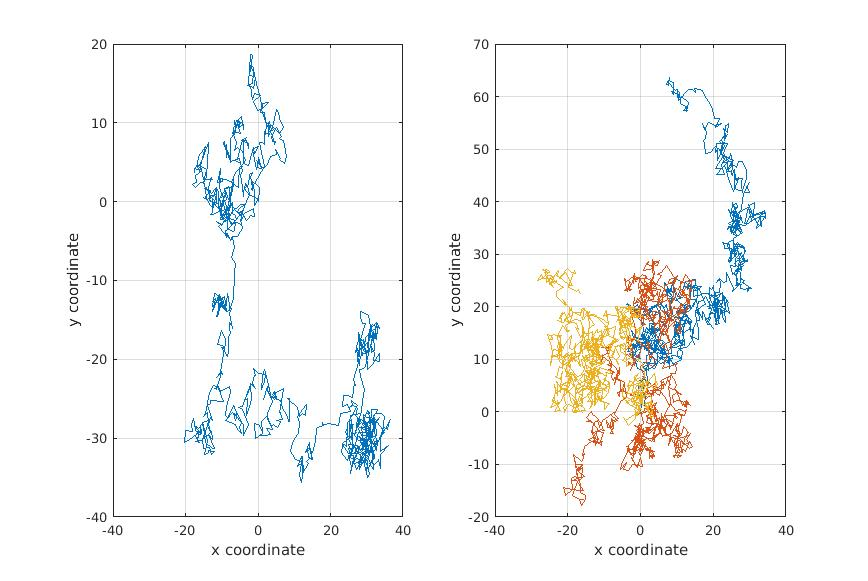
\includegraphics[width=1.0\textwidth]{brownian2d}
	\caption{Brownian simulation in 2D for one and three trajectories.}
\end{figure}

\subsection{Mean squared displacement}
Mean squared displacement is often used to measure the spatial extent of random motion. We can implement it in MATLAB to see its relationship with Brownian motion.

The code can be found below:

\begin{lstlisting}[language=Matlab, caption = {Source code for Mean squared displacement}]
function [] = mean_square(dims, timesteps, nparts)
	if dims == 1
		x =  zeros(nparts, 1);
		for i=2:timesteps
			x = [x x(:, i - 1) + randn(nparts, 1)];
		end;

		plot((sum(x.^2)/nparts)');
	elseif dims == 2
		x = zeros(nparts, 1);
		y = zeros(nparts, 1);

		for i=2:timesteps
			x = [x x(:, i - 1) + randn(nparts, 1)];
			y = [y y(:, i - 1) + randn(nparts, 1)];
		end;

		plot((sum(x.^2) + sum(y.^2))/nparts');
	else
		x = zeros(nparts, 1);
		y = zeros(nparts, 1);
		z = zeros(nparts, 1);

		for i=2:timesteps
			x = [x x(:, i - 1) + randn(nparts, 1)];
			y = [y y(:, i - 1) + randn(nparts, 1)];
			z = [z z(:, i - 1) + randn(nparts, 1)];
		end;

		plot((sum(x.^2) + sum(y.^2) + sum(z.^2))/nparts');
	end
	xlabel('timestep');
	ylabel('Mean squared displacement');
end
\end{lstlisting}

Above code has been executed for different number of dimensions and number of particles. The result can be seen on the next figure.

\begin{figure}[H]
	\centering
	\makebox[0pt]{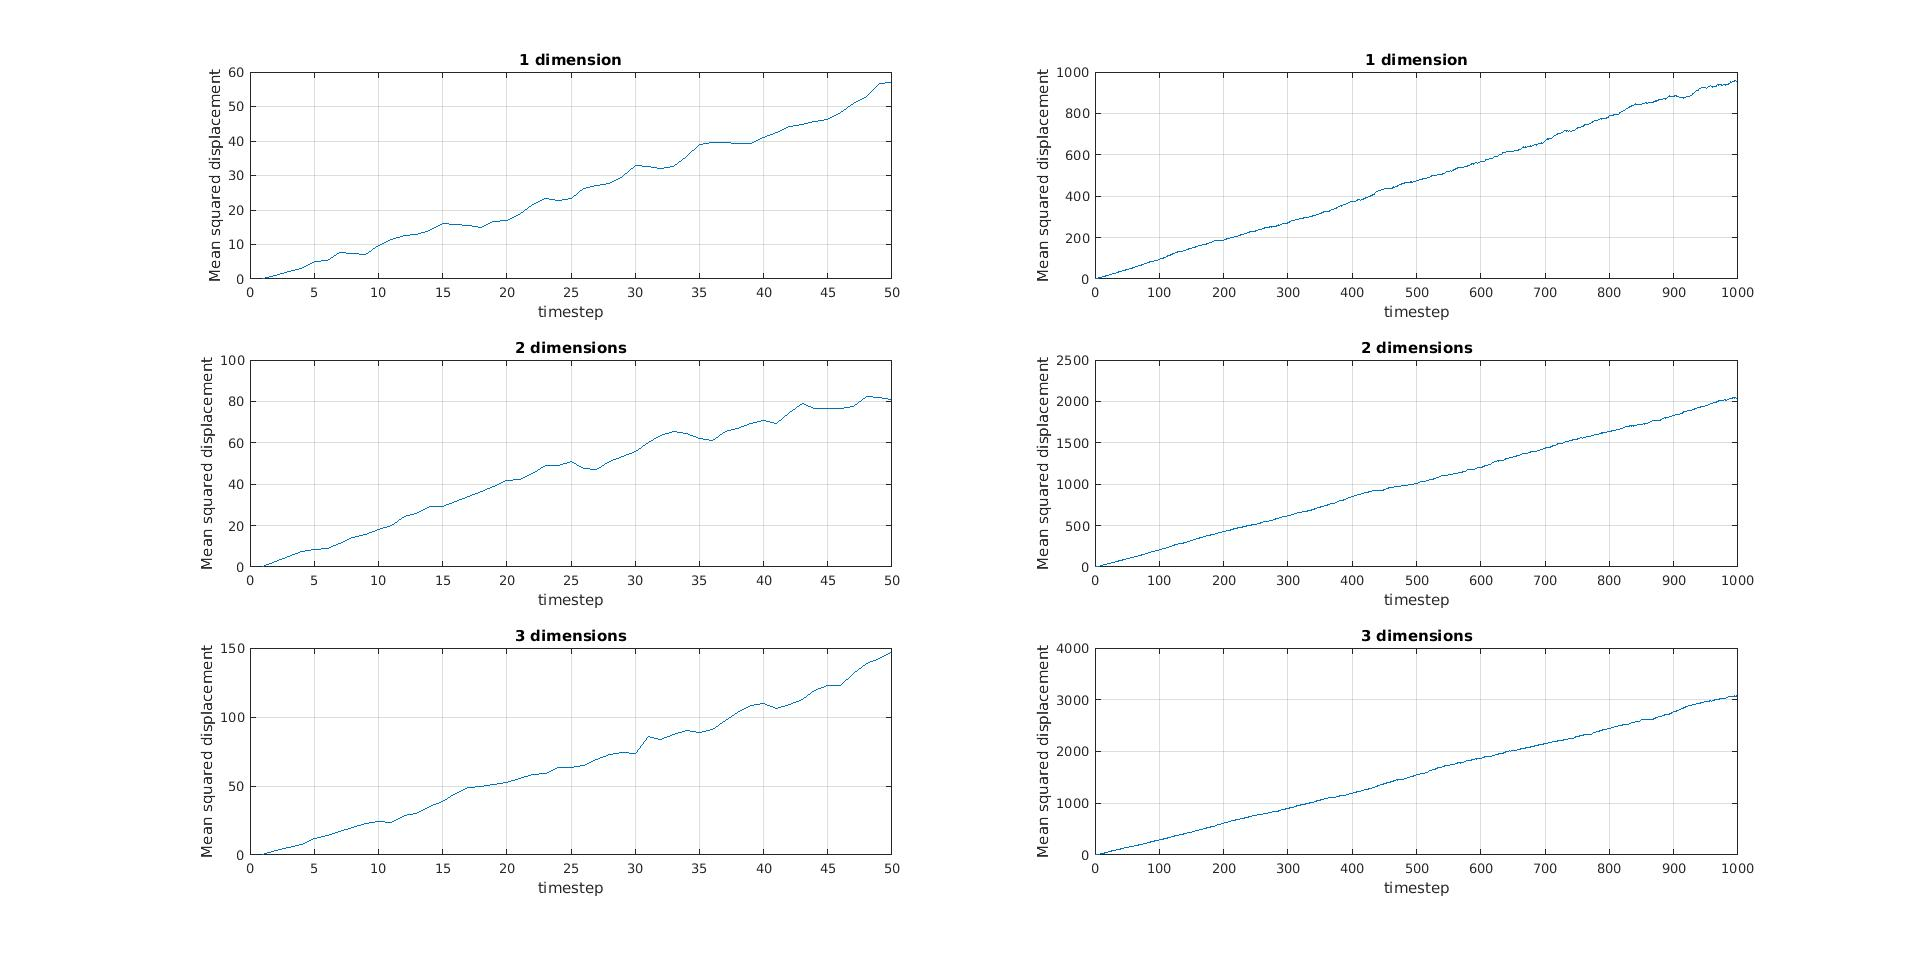
\includegraphics[width=1.45\textwidth]{mean_squared}}
	\caption{Mean squared displacement for Brownian motion.}
\end{figure}

If Brownian motion is indeed random we expect MSD to grow with time and that's exactly what happens. With bigger sample (number of particles) it looks like linear function.

\subsection{Self-similarity}
One of the Brownian motion property is \textit{self-similarity}. This property can be demonstrated using auto-correlation function as shown in the next code sample.

\begin{lstlisting}[language=Matlab, caption = {Source code for auto-correlation}]
function [] = self_similarity()

	c = [];
	a = rand(1000, 1);
	% we count correlation for random values
	for i = -49:50
		c = [c corr(a(100:900), a(100 + i:900 + i))];
	end

	subplot(2, 1, 1);
	plot(c);
	grid on;
	xlabel('x coordinate');
	ylabel('autocorrelation');
	title('Random distribution');

	x = 0;

	for i = 2:1000
		x = [x x(i - 1) + randn()];
		end

	c = [];
	% we count correlation for Brownian
	for i = -49:50
		c = [c corr(x(100:900)', x(100 + i:900 + i)')];
	end

	subplot(2, 1, 2);
	stairs(-49:50, c);

	plot(c);
	grid on;
	xlabel('x coordinate');
	ylabel('autocorrelation');
	title('Brownian motion');
end
\end{lstlisting}

This results in following plot:

\begin{figure}[H]
	\centering
	\makebox[0pt]{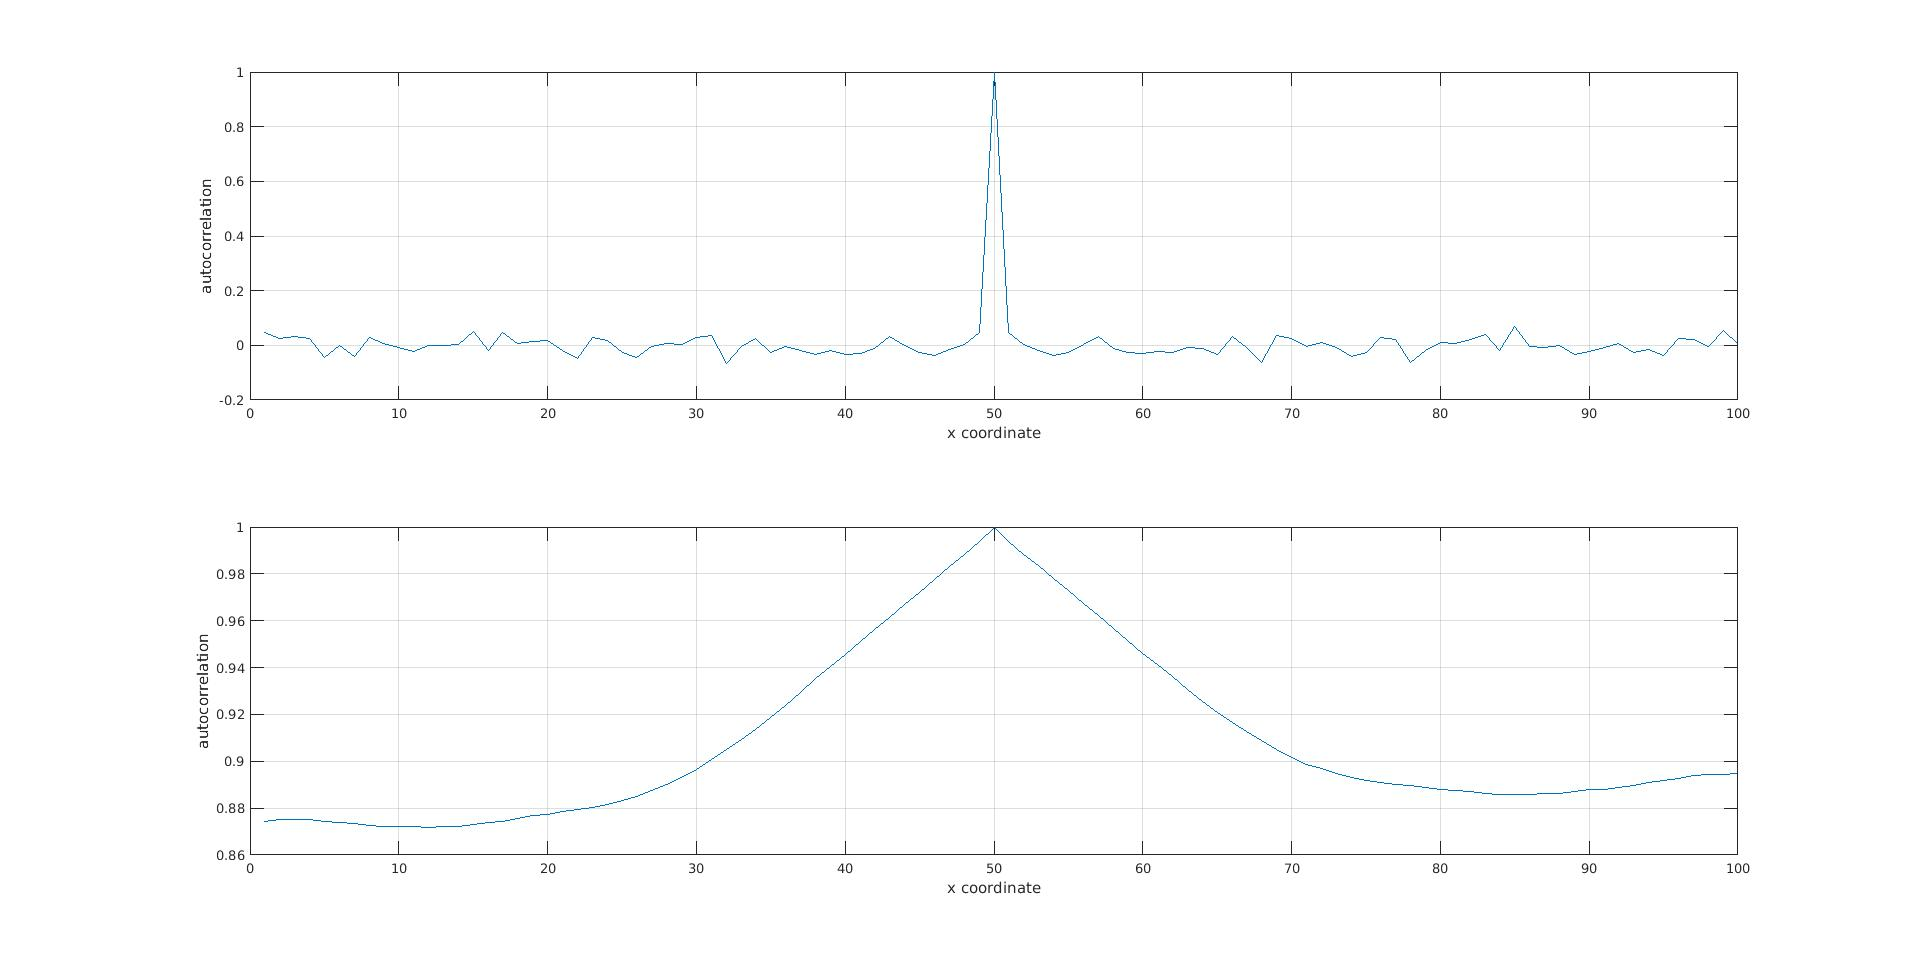
\includegraphics[width=1.4\textwidth]{auto_corr}}
	\caption{Auto-correlation for random distribution and Brownian motion.}
\end{figure}

In case of random values, the correlation factor is close to zero for most of the input. This is not the case with Brownian motion where it does not go below 0.88.

\subsection{Evolution of particles density}

We can also demonstrate time evolution of particles density starting from the same point.

\begin{lstlisting}[language=Matlab, caption = {Source code for particles density}]
function [] = particles_density(dims, timesteps, nparts)
	if dims == 1
		x =  zeros(nparts, 1);
		for i=2:timesteps
			x = [x x(:, i - 1) + randn(nparts, 1)];
		end;
		histogram(x);
		xlabel('x coordinate');
		ylabel('number of particles');

	elseif dims == 2
		x = zeros(nparts, 1);
		y = zeros(nparts, 1);

		for i=2:timesteps
			x = [x x(:, i - 1) + randn(nparts, 1)];
			y = [y y(:, i - 1) + randn(nparts, 1)];
		end;
		histogram2(x, y);
		xlabel('x coordinate');
		ylabel('y coordinate');
		zlabel('number of particles');
end
\end{lstlisting}

Next, the function is executed for both one and two dimensions.

\begin{figure}[H]
	\centering
	\makebox[0pt]{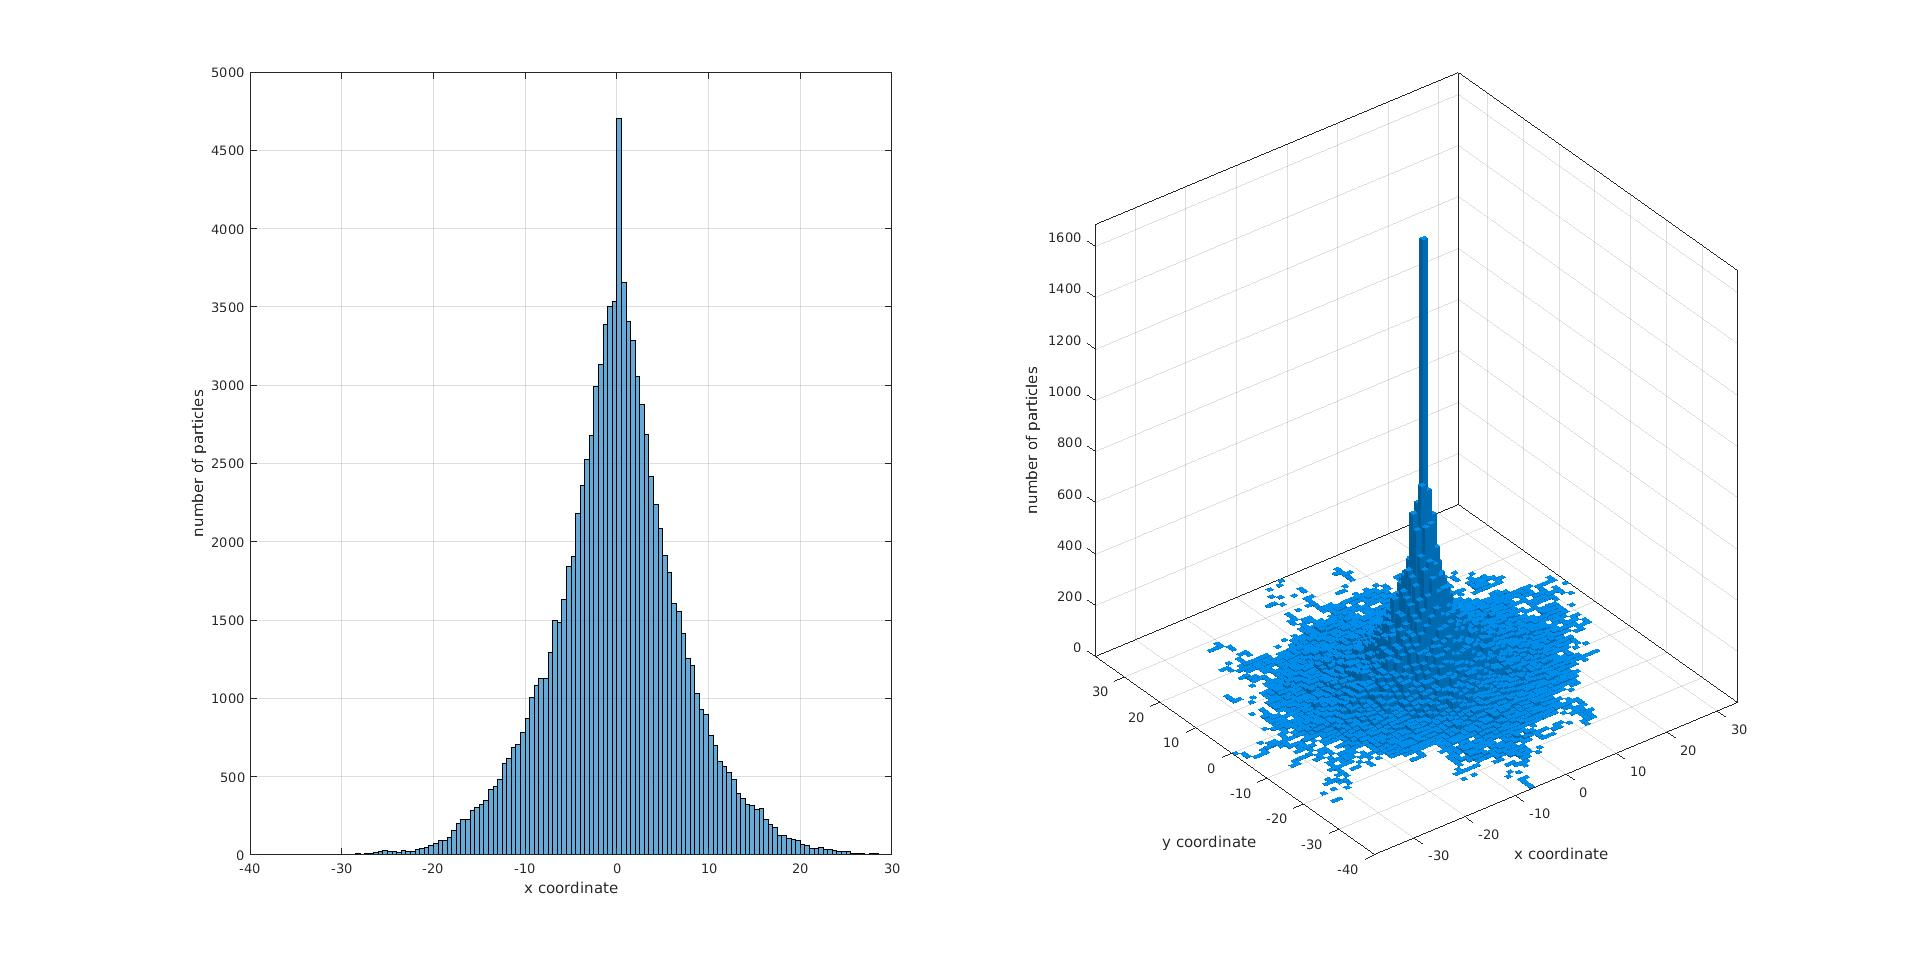
\includegraphics[width=1.4\textwidth]{particles_density}}
	\caption{Time evolution of particles density.}
\end{figure}

Looking at the figure above we notice that it looks like \textit{Gaussian Distribution} regardless of number of dimensions.


\section{Conclusion}

During this laboratory we have implemented Brownian motion in MATLAB using Monte Carlo method for acquiring random data. We have shown its \textit{self-similarity} property despite being random motion manifesting \textit{Gaussian Distribution} which is very interesting characteristic.

\subsection{Source code}

Source code using listed functions for drawing figures can be found below:

\begin{lstlisting}[language=Matlab, caption = {Source code used for drawing pictures used in this report.}]
clear; clc;

figure;
subplot(1, 2, 1);
brownian(1, 1000);
title('1 trajectory');
grid on;

subplot(1, 2, 2);
brownian(3, 1000);
title('3 trajectories');
grid on;

figure;
self_similarity();

figure;
subplot(3, 2, 1);
mean_square(1, 50, 50);
grid on;
title('1 dimension');
subplot(3, 2, 2);
mean_square(1, 1000, 1000);
grid on;
title('1 dimension');

subplot(3, 2, 3);
mean_square(2, 50, 50);
grid on;
title('2 dimensions');
subplot(3, 2, 4);
mean_square(2, 1000, 1000);
grid on;
title('2 dimensions');

subplot(3, 2, 5);
mean_square(3, 50, 50);
grid on;
title('3 dimensions');

subplot(3, 2, 6);
mean_square(3, 1000, 1000);
grid on;
title('3 dimensions');

figure;
subplot(1, 2, 1);
particles_density(1, 100, 1000);
grid on;
title('1 dimension');
subplot(1, 2, 2);
particles_density(2, 100, 1000);
title('2 dimensions');
grid on;
\end{lstlisting}


\end{document}
